
\section*{Q4: 2-approximation}

Show 2-approximation solution for TSP for the graph below.
Explain why your solution is within 2 of the optimal.

\begin{figure}[H]
    \centering
    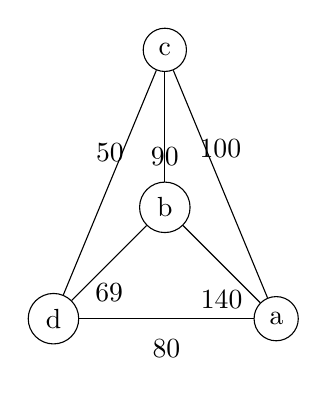
\begin{tikzpicture}[auto]
        \tikzstyle{every node} = [align=center, draw, circle, node distance = 2cm]
        \node(b){b};
        \node[above of=b](c){c};
        \node[below left of=b](d){d};
        \node[below right of=b](a){a};

        \path (a) edge node[draw=none, below](){140} (b);
        \path (a) edge node[draw=none, above](){100} (c);
        \path (a) edge node[draw=none, below](){80} (d);
        \path (b) edge node[draw=none, below](){90} (c);
        \path (b) edge node[draw=none, below](){69} (d);
        \path (c) edge node[draw=none, above](){50} (d);
    \end{tikzpicture}
\end{figure}

\subsection*{Solution}

First find Min Span Tree(MST):

\begin{figure}[H]
    \centering
    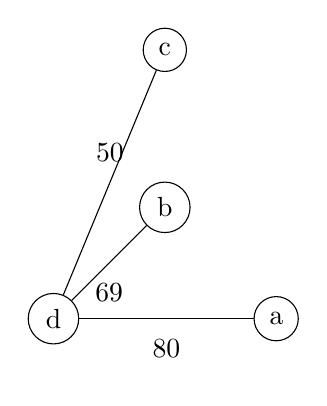
\begin{tikzpicture}[auto]
        \tikzstyle{every node} = [align=center, draw, circle, node distance = 2cm]
        \node(b){b};
        \node[above of=b](c){c};
        \node[below left of=b](d){d};
        \node[below right of=b](a){a};

        \path (a) edge node[draw=none, below](){80} (d);
        \path (b) edge node[draw=none, below](){69} (d);
        \path (c) edge node[draw=none, above](){50} (d);
    \end{tikzpicture}
\end{figure}

Suppose we use b as root.
Then our path would be:

$$ P_{MST} = b \rightarrow d \rightarrow c \rightarrow d \rightarrow a \rightarrow d \rightarrow b$$

Optimize repeated path with the 3rd path of a triangle:

$$ P_0 = b \rightarrow d \rightarrow c \rightarrow a \rightarrow b$$

Thus the cost is:

$$c(P_0) = 69+50+100+140 = 359$$

\begin{proof}
    \begin{enumerate}
        \item Our solution $c(P_0) \le 2 c(MST)$.
              It's easy to argue that $c(P_0) \le c(P_{MST})$.
              This is because we used triangle to reduced some path.
              Since $c(P_{MST}) \le 2c(MST)$, i.e. the most costy way is to traverse all path twice, back and force.
              We have $c(P_0) \le 2 c(MST)$.
        \item Suppose there is the minimum path $P_\sigma = v_k \rightarrow \cdots v_k$.
              Removing the last $v_k$ would give us a MST. Therefore $c(P_\sigma) = c(MST) + c(x, v_k) > c(MST)$
    \end{enumerate}
    Therefore we have $c(P_0) \le 2 c(MST) < 2c(P_\sigma)$
\end{proof}